% \documentclass[a4paper]{article}
\documentclass[12pt]{extarticle}
\usepackage[a4paper, left=1.5cm, right=1.5cm, top=1.5cm, bottom=2.0cm]{geometry}
\usepackage{graphicx} % Required for inserting images
\usepackage{caption}  % for continuedfloat

\usepackage{lscape} % For landscape pages
\usepackage{afterpage}
\usepackage{pdflscape} % To create landscape pages that show as landscape in PDF viewer
\usepackage{parskip} % Adds white space between paragraphs
\usepackage{amsmath}

\title{stroke\_lsoa\_prediction}
\author{Anna Laws}
\date{JuLY!!! 2025}

\begin{document}

\maketitle



\section{Introduction}

REWRITE ME.
Having an estimated number of people who will have strokes is useful for planning the hospital resources necessary.
% 
Over time, the population of the United Kingdom is increasing and aging (REFS).
As the demographics of the population change with time, the number of people having strokes should increase as more people reach older ages.
% 
There are projections of the age bands (REFS) so we can use information that is known, such as population age bands and deprivation levels, to project the expected number of admissions in future years.

suspect that stroke increases with age, so first check age bands

then also know the deprivation of the population, find that this helps to predict stroke admissions in a smaller area


We can model stroke admissions numbers as the product of the total number of people $n$ and the probability of having a stroke, $P(\textnormal{stroke})$. Then we can split the population into smaller groups and assign a different probability to each one. This allows us to give a different probability of stroke to different age groups of people, $P(\textnormal{stroke | age})$, and assume that the probability of stroke decreases with age. For five age bands (under 65, 65--70, 70--75, 75--80, 80 and over) the total number of admissions would be:

\begin{equation}
\begin{split}
    a = &P(\textnormal{stroke} | <65) \cdot n_{<65} +\\
    &P(\textnormal{stroke} | 65\textnormal{--}70) \cdot n_{65\textnormal{--}70} +\\
    &P(\textnormal{stroke} | 70\textnormal{--}75) \cdot n_{70\textnormal{--}75} +\\
    &P(\textnormal{stroke} | 75\textnormal{--}80) \cdot n_{75\textnormal{--}80} +\\
    &P(\textnormal{stroke} | \geq80) \cdot n_{\geq80}
\end{split}
\end{equation}

The Office for National Statistics provides population estimates in five-year age bands at the MSOA level. The estimates are also projected into the future so that we could estimate how stroke admissions would change over time. 

Aims: to find a formula for stroke admissions in terms of the numbers of people in the population, split by age band and by regional deprivation level.
This formula can then be applied to other areas to predict admissions even when the exact age and deprivation breakdown vs admissions is not known.
Use it to find stroke admissions in other areas and in the future.

Available data: SSNAP and HES, matching date spans.

In this document,
Steps to derive coefficients for the age-admissions prediction model:

\begin{itemize}
    \item Calculate starting coefficients from SSNAP data
    \item Genetic algorithm to explore parameter space
    \item Optimisation with simulated annealing to find precise fits
\end{itemize}



Want to predict number of stroke admissions when we know only the population demographics, specifically the number of people of various ages. Assume that in general older people are more likely to have strokes than younger people and so the age breakdown matters. Use the age bands: under 65, 65 to 70, 70 to 75, 75 to 80, and over 80.

Data available at the MSOA level:
+ number of admissions from 2017 to 2019, from Hospital Episode Statistics (HES).
+ number of people in each age band in mid-2020.
+ deprivation ranking (Index of Multiple Deprivation, IMD).

Data available at the national level:
+ number of stroke admissions from people in each age band from 2017 to 2019, from the Sentinel Stroke National Audit Programme (SSNAP).
+ number of people in each age band in January 2019.

Start by using the national-level data to find the pattern of stroke incidence with age, and then use the MSOA-level data to add in deprivation level.


\section{Method}

In the MSOA-level admissions and demographic data we find that there is a good correlation between the number of people in the older age bands (age over 65) and the admissions numbers. The correlation becomes stronger when the MSOA are split by deprivation ranking. The more deprived areas are associated with more stroke admissions than less deprived areas.

In Figure~\ref{fig:scatter_age_admissions_by_imd}, the data from all MSOA is shown in every panel in grey. Then the data from only MSOA in the given deprivation quantile is overplotted in a colour. The x-axis shows the number of people in each age band in an MSOA and the y-axis shows the total number of admissions from each MSOA (note: the admissions are the total from all age bands, not just the age band relevant that to each panel).
The data for the most deprived quantiles (top row, purple points) tend to appear further left and higher up than the least deprived quantiles (bottom row, yellow points). This means that in more deprived areas, fewer people are needed in the older age groups to reach the same number of stroke admissions as in the less deprived areas. In other words, the probability of stroke is higher in more deprived areas.

\subsection{Stroke risk with age}

We can use SSNAP audit data for all strokes in England that were recorded on the stroke pathway and calculate estimates of the probability of stroke for each age band. We know both the numbers of people having strokes and can place them into the required five-year age band at the time of stroke.

We also have HES admissions data that includes all recorded stroke including some outside the usual stroke pathway that do not appear in SSNAP data. The HES data is available at MSOA level for 2017 to 2019 inclusive and seems to only be valid for English MSOA.
To take a subset of the SSNAP data that is a good match to HES, we can limit the date range to 2017 to 2019 inclusive and keep admissions to English hospitals only, assuming that patients based in Welsh MSOA only go to Welsh hospitals.

To convert the SSNAP data to annual stroke admissions, divide the total number of strokes in each age band by three for the three years 2017 to 2019 and then scale up the results by the ratio of the total admissions in the HES and in the SSNAP data, which is around 1.45.

We then take England population data from January 2019 and combine it into the same five age bands as the admissions.
This allows us to compare the numbers of patients in each age band with the numbers of admissions and calculatte the probabilitie sof stroke in Table~\ref{tab:ssnap_coeffs}.


\begin{table}
\centering
    \caption{Stroke coefficients from SSNAP data. England population is 56.3 million in January 2019 and total annual strokes are 80,958.}
    \begin{tabular}{crrr}
    Age Groups & Percentage of all population & Annual admissions & Probability of stroke given age \\
    \hline
    Less than 65 & 81.6\% & 18737.7 & 0.04\% \\
    65--69 & 5.0\% & 7395.3 & 0.26\% \\
    70--74 & 5.0\% & 10379.6 & 0.37\% \\
    75--79 & 3.4\% & 11654.6 & 0.60\% \\
    80+ & 5.0\% & 32790.8 & 1.16\% \\
    \end{tabular}
    \label{tab:ssnap_coeffs}
\end{table}

\begin{figure}
    \centering
    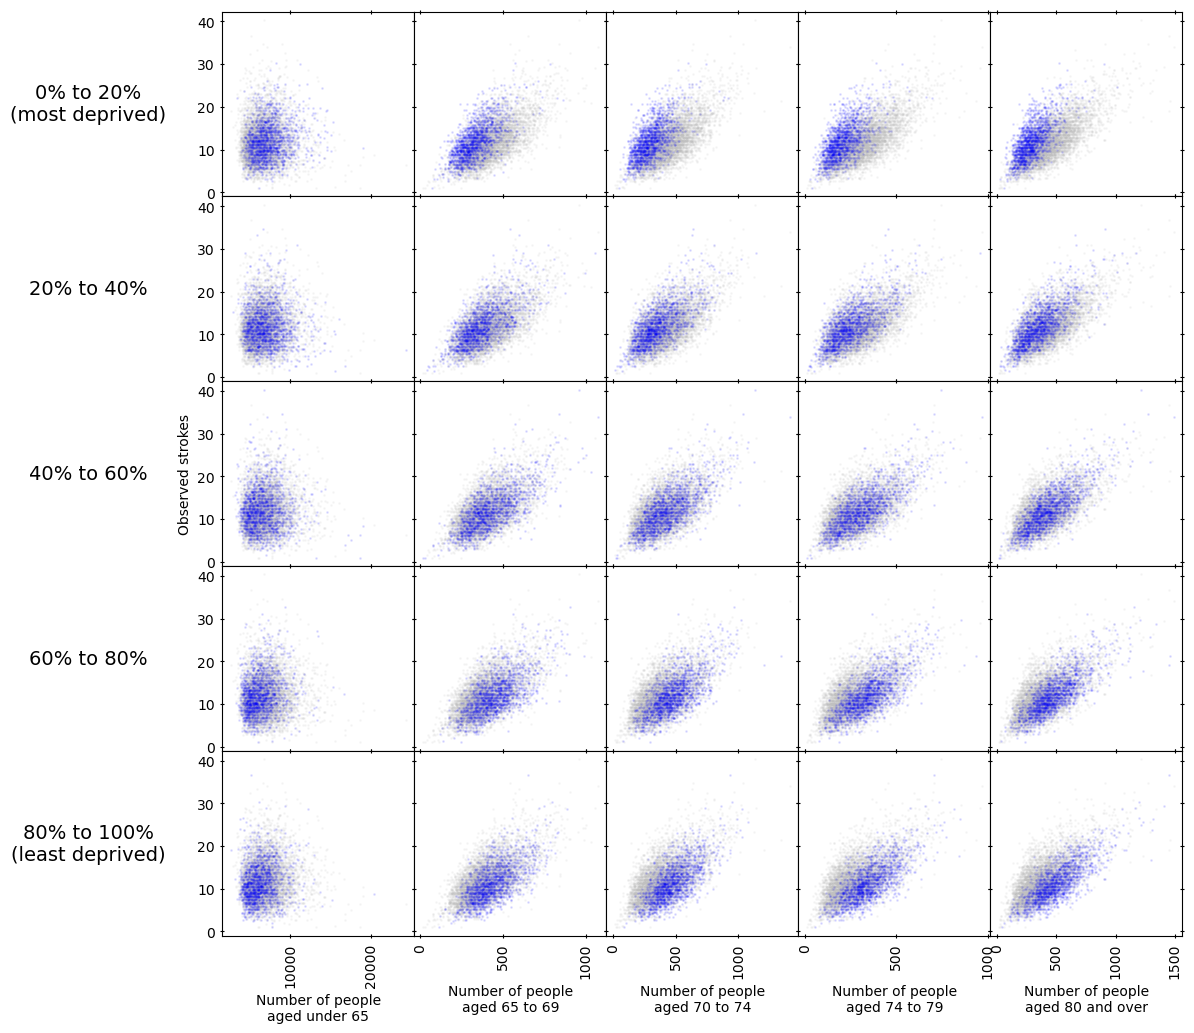
\includegraphics[width=1.0\linewidth]{images/scatter_age_admissions_by_imd.png}
    \caption{Comparison of the numbers of people in each age band with the number of admissions for each MSOA, split by deprivation level. The grey markers show data for all MSOA in all cases and coloured markers show the data for only MSOA in the stated deprivation level.}
    \label{fig:scatter_age_admissions_by_imd}
\end{figure}


\begin{figure}
    \centering
    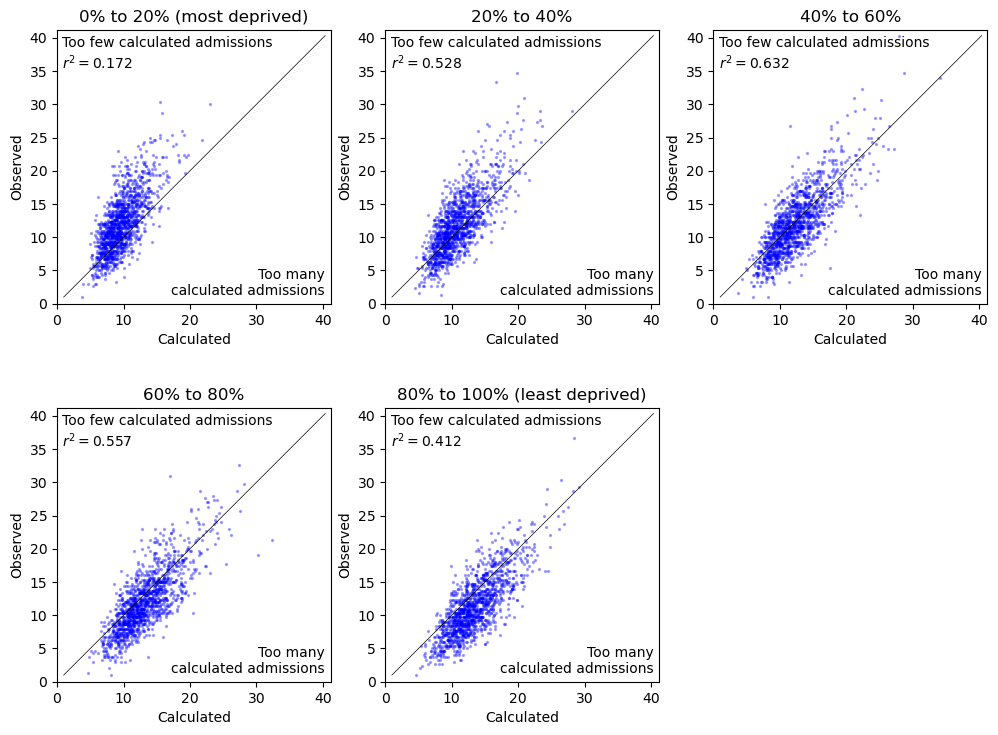
\includegraphics[width=1.0\linewidth]{images/scatter_admissions_from_ssnap_coeffs_separate.png}
    \caption{Comparison of the numbers of admissions calculated using the age-band-derived coefficients with the observed admissions in each MSOA, split by deprivation level. The black diagonal line marks where the two measures are equal.}
    \label{fig:scatter_admissions_from_ssnap_coeffs_separate}
\end{figure}

We can use these SSNAP coefficients with the MSOA-level population data to calculate the numbers of annual admissions from each MSOA and compare the closeness of fit to the observed admissions data.
The results are shown in Figure~\ref{fig:scatter_admissions} (left panel). The r-squared value of the calculated to observed admissions is 0.455. 


We have insufficient data to directly calculate the probability of stroke given age band and deprivation level. We have data for the number of admissions in each age band, and the number of admissions from each deprivation level, but not the data for each combination of age band and deprivation level.

First we can calculate the effect on admissions from just age band.
The SSNAP data contains the total number of admissions for each of the above age groups. We can combine this with the total number of people in England in each age band. This gives an estimate of the probability of stroke given a certain age band.


We can judge the accuracy of these coefficients by using them with the MSOA-level population data to calculate the number of admissions in each MSOA.
The results can be compared with the observed numbers of admissions in each MSOA from the HES data.

The following scatter plot compares the observed and calculated admissions numbers for all MSOA. It has a black line where the two values are equal. Data points appearing above that line have more calculated than observed admissions, and points below the line have fewer.

Figure~\ref{fig:scatter_admissions_from_ssnap_coeffs_separate} shows the admissions for each MSOA where MSOAs are coloured by their deprivation score quantile. 
All MSOA are placed into one of five groups according to their rank of most to least deprived MSOAs.
The scatter shows that MSOA in the most deprived groups fall below the line where calculated admissions are identical to observed, and so the most deprived MSOA have more admissions in reality than predicted by the model.
Similarly the least deprived MSOA have fewer admissions than predicted.
This means that a better predictor of annual admissions numbers at the MSOA level should be found if the MSOA's deprivation quantile is taken into account, and different deprivation quantiles are allowed different probabilities of stroke.


We see that the admission numbers are largely under-predicted for the most-deprived MSOAs and slightly over-predicted for the least-deprived MSOAs.

The calculations could be made more accurate by using different coefficients for each deprivation group.
The SSNAP data does not contain the patients' MSOA names and so the admissions cannot be linked to deprivation index directly.
However we can use these derived coefficients as a starting point for finding a new fit using the deprivation data.

\subsection{Stroke risk with deprivation}


We can find values for coefficients split by age band and by deprivation level by using an optimiser.
In this case we can't directly calculate the coefficients from the HES data because the observed admission numbers will contain random errors.
The HES data covers only three years and so we expect that by chance some MSOA will have recorded more than the true average and others less than the true average.
This effect wasn't so important with the SSNAP data, which was on the national level, but with typically around 10 annual admissions per MSOA the effect can make a large difference in the HES data.
Therefore the goal is to find a set of coefficients that makes the best possible match to all MSOA simultaneously.

Optimisers require a decent first estimate of the coefficients: the closer the better, and in particular they need to be to the right order of magnitude. Otherwise it's "garbage in, garbage out". For the first estimates, we'll use variations of the coefficients derived from the SSNAP data alone.

We'll use two stages of optimisation:
1. a genetic algorithm to explore a large number of combinations of coefficients, and
2. a minimisation function to increase the precision of the results of the genetic algorithm.



\subsubsection{Genetic algorithm}

We can use the genetic algorithm to compare many sets of coefficients, select the best, and combine sets to create brand-new sets. This allows us to explore as much parameter space (try as many combinations of coefficients) as possible.

% %%%%% FITNESS %%%%%
The fitness of a set of coefficients is judged by:
+ calculating the difference between predicted and observed total admissions, then
+ scaling these by a "wrongness factor" derived from comparing the predicted and observed admissions in each age band.

The "wrongness factor" discourages the preference for sets of coefficients where most values are zero and only the values for one or two age bands are fine-tuned to make a good match for the total admissions. 

The fitness of a set of coefficients is evaluated by calculating the admissions across all MSOA and comparing it with the observed total value. The closeness is calculated by combining the sum of square residuals in admissions across all MSOA with a ``wrongness factor'' derived from how far off the admissions are in each age band.
This ``wrongness factor'' prevents the case where one age band has many more and another age band many fewer admissions than observed so that the total amount is close to correct, but the individual age bands are far from correct.
The factor is derived by calculating the total admissions in each age band, then taking the ratio of these to the observed admissions, taking the absolute difference of each ratio from the perfect 1 score, and then summing the five differences. This combined score is then added to one and multiplied by the sum of square residuals so far.
The absolute difference is used so that the same penalty applies for calculating too few as too many admissions.



% %%%%% STARTING OPTIONS %%%%%

In the genetic algorithm we define coefficients in terms of the scale values for the SSNAP coefficients rather than the actual values themselvesl. This makes the mutations easier because the scales are similar values but the actual coefficients are different orders of magnitude so it's trickier to scale them fairly in the same way.

The genetic algorithm starts with 300 "individuals" or sets of coefficients. These are picked from 2002 options. The options are various combinations of scaled values of the SSNAP coefficients: for example, the most-deprived areas might use the starting values multiplied by 1.4, the least-deprived areas 0.6, and the other areas scales in between.

There are some conditions imposed on the sets of coefficients.
We assume that probability of stroke should increase with age, as was seen with the SSNAP-derived coefficients, and with deprivation. Any sets of coefficients that are generated are adjusted if necessary so that these conditions are always met.


Start with the SSNAP-derived coefficients in Table~\ref{tab:ssnap_coeffs}.
Assume that different IMD quantiles will have different coefficients, and in particular that more-deprived quantiles will have higher coefficients (higher probability of stroke). 
Allow starting coefficients for each IMD band to be the SSNAP coefficients multiplied by a scaling factor in 0.2 to 2.0 in steps of 0.2.
First calculate all combinations of these scale factors for the five IMD bands, then only keep combinations where the scale factor is larger in more-deprived quantiles.
The range 0.2 to 2.0 was used because test optimisation cases never found good fits with scale factors outside this range.

For five quantiles in the order most deprived to least deprived, the final combinations are:
\begin{itemize}
    \item 0.2, 0.2, 0.2, 0.2, 0.2,
    \item 0.4, 0.2, 0.2, 0.2, 0.2,
    \item 0.4, 0.4, 0.2, 0.2, 0.2,
    \item 0.4, 0.4, 0.4, 0.2, 0.2,
    \item 0.4, 0.4, 0.4, 0.4, 0.2,
    \item ...
    \item 2. , 2. , 2. , 2. , 1.2,
    \item 2. , 2. , 2. , 2. , 1.4,
    \item 2. , 2. , 2. , 2. , 1.6,
    \item 2. , 2. , 2. , 2. , 1.8,
     \item 2. , 2. , 2. , 2. , 2.
\end{itemize}
There are 2002 options in total.

Some of these starting combinations would give wildly inaccurate total admissions, for example when all scales are much larger or less than 1, but using the genetic algorithm we can easily create a new generation of individuals that have a better mix of large and small scales.



% %%%%% RUNNING DEAP %%%%%

We use DEAP to create the genetic algorithm.


In each generation of the algorithm, the individuals are paired up and given a chance of swapping over a random string of their coefficients (crossover). Then the individuals have a chance of their coefficients being nudged slightly, for example from a scale of 1.4 to 1.32 (mutation). The algorithm uses high mutation and crossover rates to sample as much variation in the coefficient values as possible.
Then a set of individuals are picked out to continue to the next generation with better sets of coefficients (according to the fitness tests) being more likely to be picked.


Encourage high mutation and crossover rates to get as much variation, explore as much parameter space as possible.
But for an individual that mutates, only 4\% chance of each coeff changing - so on average expect a mutating individual to have only one, maybe zero or two coeffs mutate.
On mutation, new coefficients are picked using a Gaussian distribution with mean 0 and std of 0.1, large enough so that mutations can easily reach a value of plus or minus 0.1 from the current value.

We use 100 random seeds to run 100 different starting populations.
In each run, a population of available stroke coefficients is created by selecting 300 individuals from the available 2002 starting sets.
The algorithm runs for 1000 generations or until the std in all coefficients is less than 5\% of the mean value, as an approximation for when most of the individuals contain mostly similar values. 


We run the simulation 100 times with different selections of starting individuals each time. We keep a copy of the best individual from the final generation of each of the 100 simulations.

The simulation continues until either 1000 generations have passed or all of the individuals have similar coefficients (standard deviation is less than 5\% of the mean for each coefficient). When all individuals are so similar, there is not much further improvement to be gained from crossover.


% %%%%% RESULTS %%%%%
The resulting best individuals all have r-squared over 0.57. Five of them have r-squared values that round to 0.592.


\begin{figure}
    \centering
    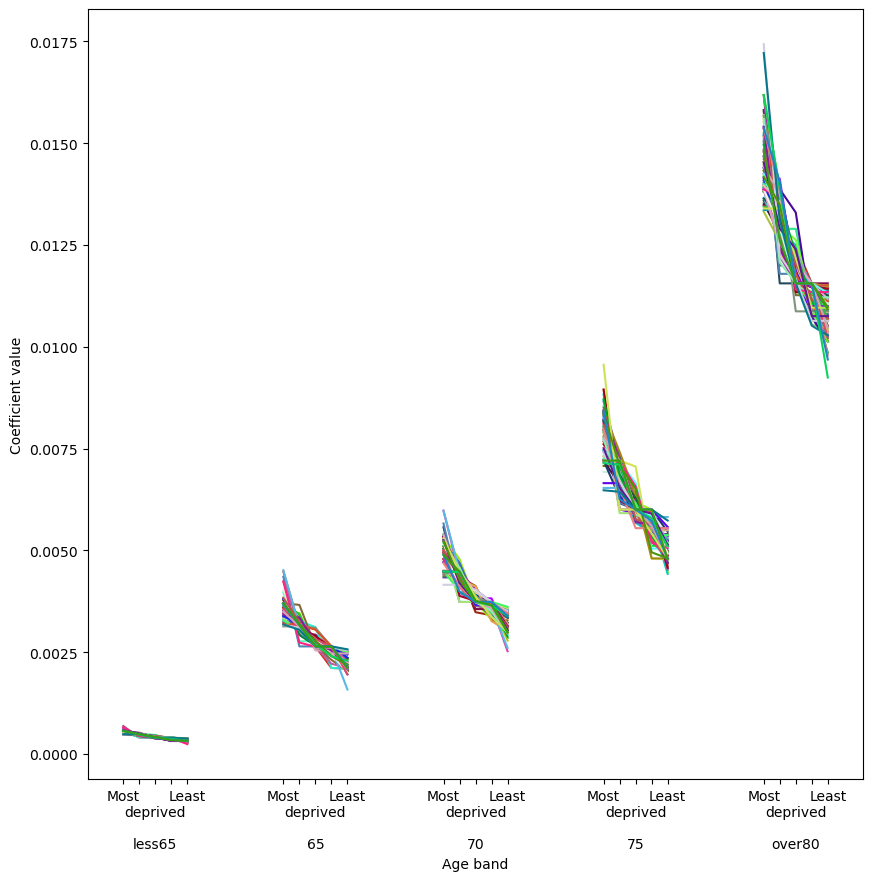
\includegraphics[width=1.0\linewidth]{images/scatter_coeffs_from_deap.png}
    \caption{Line plots of the 100 sets of coefficients found from the genetic algorithm.}
    \label{fig:scatter_coeffs_from_deap}
\end{figure}


The resulting best 100 individuals are shown in Figure~\ref{fig:scatter_coeffs_from_deap} as a way to judge how similar the results are. Each of the 100 sets of coefficients has a different colour.
% 
The 100 sets of coefficients have not converged on a single set of consistently good values. Even when rounded to one significant figure, the results are not consistent.

To see if the results will converge, we can use a second optimisation step to increase the precision of the coefficients.


\subsubsection{Simulated annealing}



The minimisation function takes a set of coefficients and adjusts the values to find the set that minimises the error in some function. In this case, it will minimise the difference between calculated and observed total admissions (modified by the "wrongness factor").
Because it is unlikely that the genetic algorithm would have generated the best coefficients by chance, the minimisation can take each of the 100 sets of coefficients and fine-tune them to the best possible combination that is near these starting values.

Minimisation works best when the initial guess is close to the true best values. However, the results of the genetic algorithm did not converge to a small set of values. This could mean that there are a large number of sets of coefficients that give very good results (there are many local minima). To increase the chances of finding the true best values (global minimum), we use simulated annealing. This basically allows the optimiser to consider using a set of coefficients that is not quite as good as its last attempt, but that has the potential to be fine-tuned to something even better.


% %%%%% INPUTS %%%%%
The minimisation is run separately on each of the 100 sets of best coefficients from the genetic algorithm simulations.

Use the 100 results from the genetic algorithms as the starting points for simulated annealing. This will take each set of coefficients and find a more precise set that gives the best available r-squared.

The optimisation runs on the actual coefficients rather than the scale factors as before because it is difficult to edit the input parameters and then return them from the optimiser. Instead another penalty is applied to the evaluation metric if the coefficients don't increase nicely with age and with deprivation quantile. The penalty is calculated by finding the total number of coefficients that break each pattern (increase with age, increase with deprivation), multiplying this by 0.2, and then multiplying that scale factor by the current sum of square residuals.
Practically this means that otherwise good fits that break the expected pattern should never be favoured over fits that behave.

% %%%%% METHOD %%%%%

The simulated annealing is run with temperature 30 and step size 5e-5.
The temperature is chosen from eyeballing the difference in sum of square residuals between a good first estimate and an optimised set of coefficients, so this temperature should allow a hop into the next basin.
The step size is chosen from trial and error. It seems to allow best r-squared values to be found from the optimised results. Otherwise when the step is too big, it is maybe too big for the under 65 age band with the smallest coeffs, and when it is too small, the function doesn't seem to be able to hop between basins well.


% %%%%% RESULTS %%%%%
The results of the annealing are 100 sets of coefficients, only one of which has an r-squared rounding to the maximum value of 0.593.
We use this set of coefficients to one or two significant figures as the ``best'' and use the rest as an indication of the likely range of values.
We justify this because the values aren't converging so don't trust that the extra precision in the coefficients will give a better answer overall.
The chosen final coefficients are in Table~\ref{tab:best_coeffs}.


\begin{table}
\centering
\caption{Derived coefficients: probability of having a stroke given age band and deprivation quantile.}
\begin{tabular}{llllll}
Depriv. quantile min. & less65 & 65-70 & 70-75 & 75-80 & over80 \\
\hline
0.0 (most) & 0.06\% & 0.3\% & 0.7\% & 0.7\% & 1.2\% \\
0.2 & 0.05\% & 0.3\% & 0.5\% & 0.6\% & 1.2\% \\
0.4 & 0.04\% & 0.3\% & 0.3\% & 0.6\% & 1.2\% \\
0.6 & 0.04\% & 0.3\% & 0.3\% & 0.6\% & 1.2\% \\
0.8 (least) & 0.02\% & 0.2\% & 0.3\% & 0.6\% & 1.2\% \\
\end{tabular}
\label{tab:best_coeffs}
\end{table}


We find 100 sets of minimised values.
They still haven't converged onto one set of coefficients!
This implies that there are many combinations of coefficients that are all pretty much as good as each other.
In that case, there's no sense in reporting the coefficients too precisely because we know that any small adjustment in values won't drastically affect the accuracy of the results. Instead we only keep the coefficients to one significant figure for all age bands except the over 80 band, which has two significant figures because its values are typically an order of magnitude larger than most of the others.

Before rounding, we calculate the r-squared values to assess the accuracy of the calculated vs observed admission numbers for each of the 100 sets of results.
One of these sets has a slightly higher r-squared value than the rest: it is the only r-squared value that rounds to 0.594.
However all 100 results have r-squared values that round to 0.591 or higher.

We use the best set of coefficients as the final values and use the complete set of 100 sets to judge their precision using the range of values of each coefficient.


\section{Results}

\subsection{Applying resulting coefficients}


\begin{figure}
    \centering
    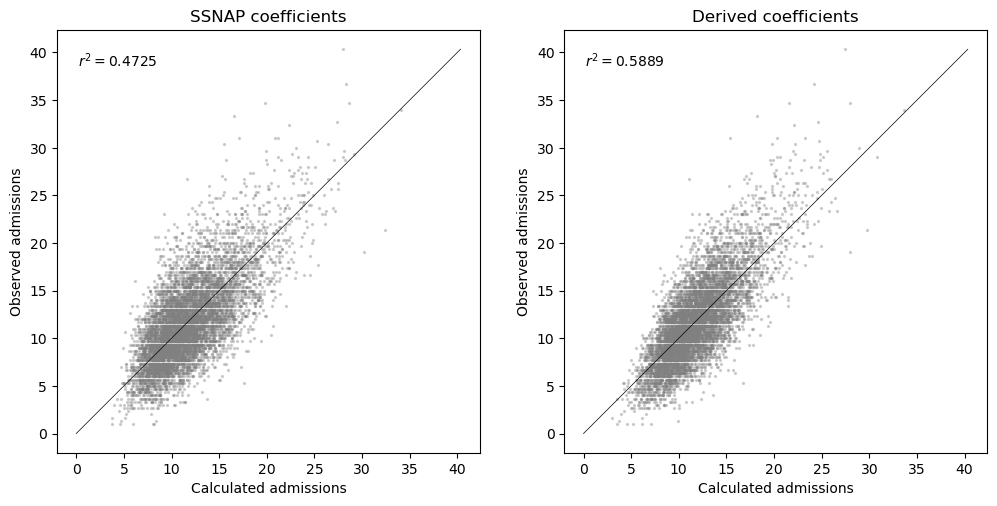
\includegraphics[width=1.0\linewidth]{images/admissions_prediction_comparison.png}
    \caption{Comparison of the numbers of admissions calculated using the age-band-derived coefficients (left panel) and the deprivation-derived coefficients (right panel) with the observed admissions in each MSOA. The black diagonal line marks where the two measures are equal.}
    \label{fig:admissions_prediction_comparison}
\end{figure}


\begin{figure}
    \centering
    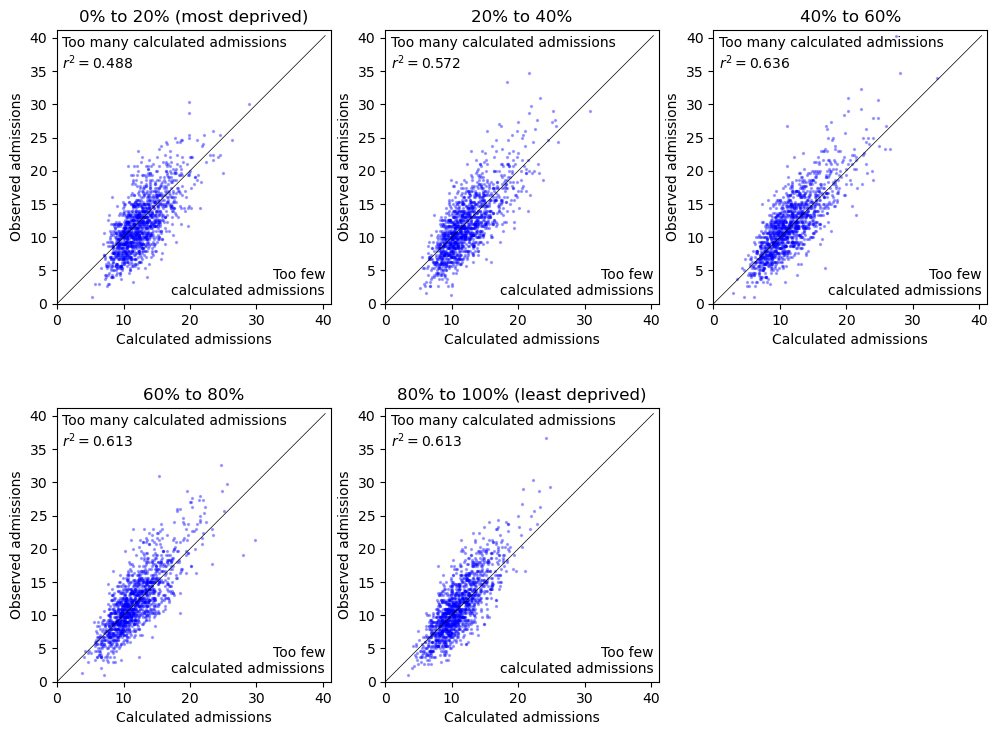
\includegraphics[width=1.0\linewidth]{images/admissions_prediction_comparison_separate.png}
    \caption{Comparison of the numbers of admissions calculated using the deprivation-derived coefficients with the observed admissions in each MSOA, split by deprivation level. The black diagonal line marks where the two measures are equal.}
    \label{fig:admissions_prediction_comparison_separate}
\end{figure}


\begin{table}
\centering
\caption{Coefficient performance. Sum of square residuals excludes any penalties and wrongness factors.}
\begin{tabular}{llll}
Coefficients set & Sum of square residuals & R-squared & Admissions \\
\hline
SSNAP & 274.931 & 0.455 & 77467.1 \\
Best & 238.884 & 0.589 & 80597.9 \\
Minimum & 262.6 & 0.503 & 72617.8 \\
Maximum & 272.36 & 0.465 & 91071.4 \\
\end{tabular}
\label{tab:coeff_performance}
\end{table}


% %%%%% R-SQUARED %%%%%
We can use these coefficients to calculate the admissions for each MSOA and see whether the accuracy has improved compared with the starting SSNAP-derived coefficients.

Figure~\ref{fig:admissions_prediction_comparison} shows the admissions for all MSOA.
There is less variation from the equality diagonal line for the derived coefficients than for the SSNAP coefficients. The r-squared values have also increased from 0.46 for the SSNAP-derived coefficients to 0.59 for these coefficients.

Figure~\ref{fig:admissions_prediction_comparison_separate} contain the same data as above but split into separate panels for each deprivation quantile.
While previously there was a noticeably worse fit for the more-deprived areas, this effect has reduced when using the final coefficients. For example, the r-squared value for only the most-deprived areas was previously 0.01 (atrocious!) and is now 0.49 (better!).

% %%%%% TOTAL ADMISSIONS %%%%%
Comparison of coefficient performance in Table~\ref{tab:coeff_performance}.

The min/max values are more extreme than any individual of the 100 found sets of coefficients because they use the largest/smallest value seen for each coefficient across all 100 fits, not taking into account that fits will have a balance of large and small coefficients to make the total admissions match the required value.
So comparing the total admissions calculated in Table~\ref{tab:coeff_performance} with the observed value, 80958.0, we can say that the calculated admissions numbers are accurate to plus or minus 10\%.

The "minimum coeffs" and "maximum coeffs" columns use the smallest and largest coefficients in the range of values given in the final results table.
This gives a worst-case scenario for the accuracy of the admissions numbers.
We see that using this extreme range of values adds or subtracts around 10\% from the admissions numbers for the "best" coefficients.


% %%%%% APPLY WRONG DEPRIVATION COEFFS %%%%%
As a further test of the derived coefficients, we can compare the admissions numbers when we deliberately use the wrong set of coefficients.
We pick out an MSOA in the middle deprivation quantile and with populations in each age band of 6710, 476, 450, 360, and 528 for the under 65, 65 to 69, 70 to 74, 75 to 79, and over 80 age bands respectively, and observed annual admissions numbers of 14.3.
% 
Using the final coefficients for each deprivation level from most to least deprived we calculate the following numbers of admissions: 17.5, 15.5, 14.0, 14.0, and 12.1.
%
So applying the coefficients from the wrong deprivation quantile should make the difference of a handful of admissions.

\section{Discussion}

There is a link between the numbers of patients with good/fair/bad health and admission numbers. However the age data is known more accurately and completely and can more easily be projected into the future than health levels.

The admissions and population data from multiple MSOA in the same deprivation quantile could be summed to create larger arbitrary areas and so reduce the effect of unusual observations (admissions in the observed years being much higher or lower than typical). This idea was excluded from the final analysis because it added a layer of complication without an obvious benefit to the results.


Variation with deprivation, age expected?

Application to other populations, e.g. other country data.

Application to other population projections, e.g. future population.

Accuracy and significant figures.


Example: England in the future.

Example: some invented population, compare admissions for same pop numbers across the depriv bands. How much difference do the depriv bands make? Coeffs small, balanced by populations large, might make a difference of a few admissions annually.


\section{Conclusion}

We have derived a set of coefficients that allow a calculation of admission numbers for stroke from a population given its deprivation level and the number of people in each age band.

\end{document}
